\chapter{机器学习方法}

首先,我们对原始数据集随机取样其60\%记录作为我们的训练集,其余40\%作为测试集。然后,分别利用逻辑回归、
分类树以及随机森林对于训练集进行监督式学习,得到相应的分类器。

\section{逻辑回归}
\subsection{逻辑回归简介}

传统的线性回归$y = \theta x$(其中$\theta$为特征变量的系数行向量,$x$为特征变量列向量)所得到的因变量$y$
的取值范围往往在整个实数空间内,而一般的分类问题只有可数个因变量取值。逻辑回归利用逻辑函数$h(z) = \frac{1}{1+e^{-z}}$(其中$z=\theta x$)将实数空间内的数映射到[0, 1]上,使得连续问题转化为离散问题的``概率''解(见图\ref{fig:logistic})。

\begin{figure}
\centering
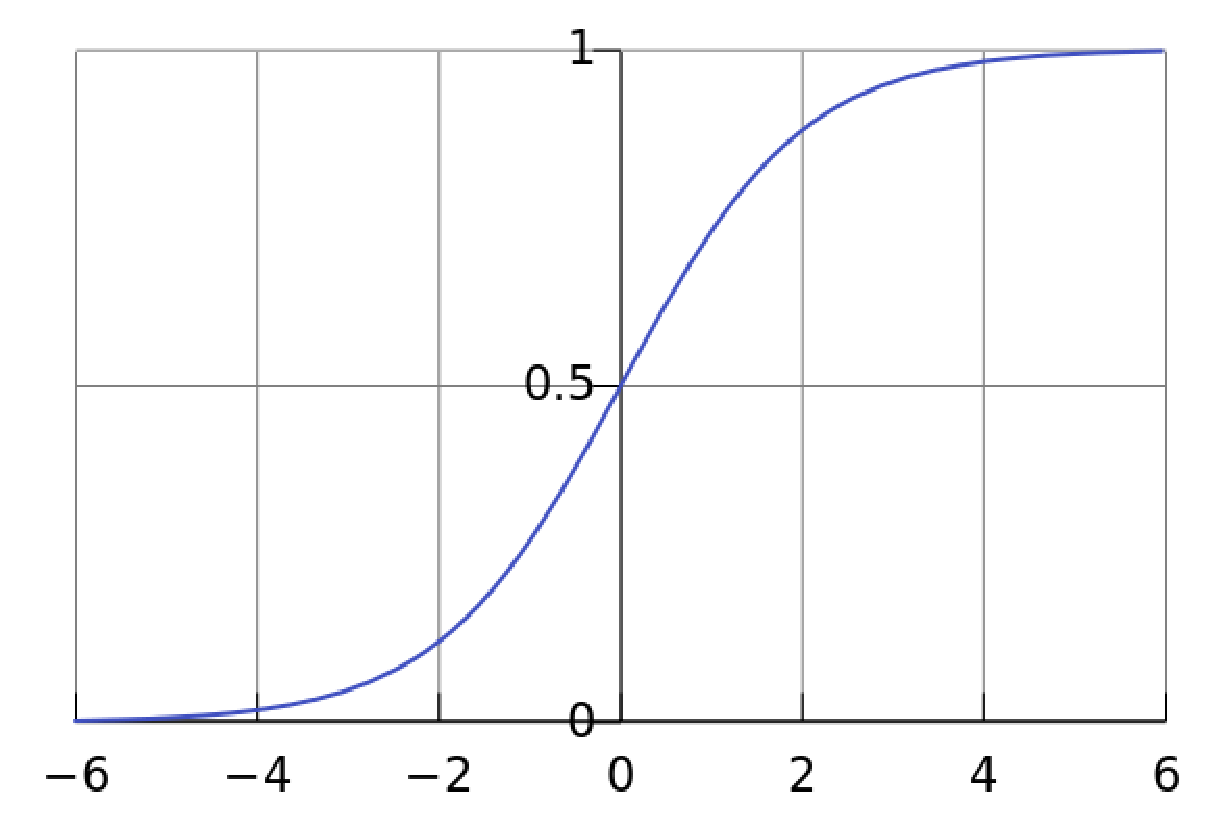
\includegraphics[width=0.8\linewidth]{logit.pdf}
\caption{\label{fig:logistic}逻辑函数}
\end{figure}

\subsection{逻辑回归算法}
其合理性是由于在分界线(面,见图\ref{fig:bound})上的数据点的$z$值为0,通过逻辑函数映射到0.5,代表分解线(面)上的数据点
无法判断其类别,可以理解为有50\%的概率为Negative Class,有50\%的概率为Positive Class;分界线(面)把多维空间
分为了两个部分,其中正向空间内离分界线(面)越远$z$值越大,通过逻辑函数映射到1,代表正向空间内远离分界线(面)
的数据点有很大的可能性为Positive Class。

\begin{figure}
\centering
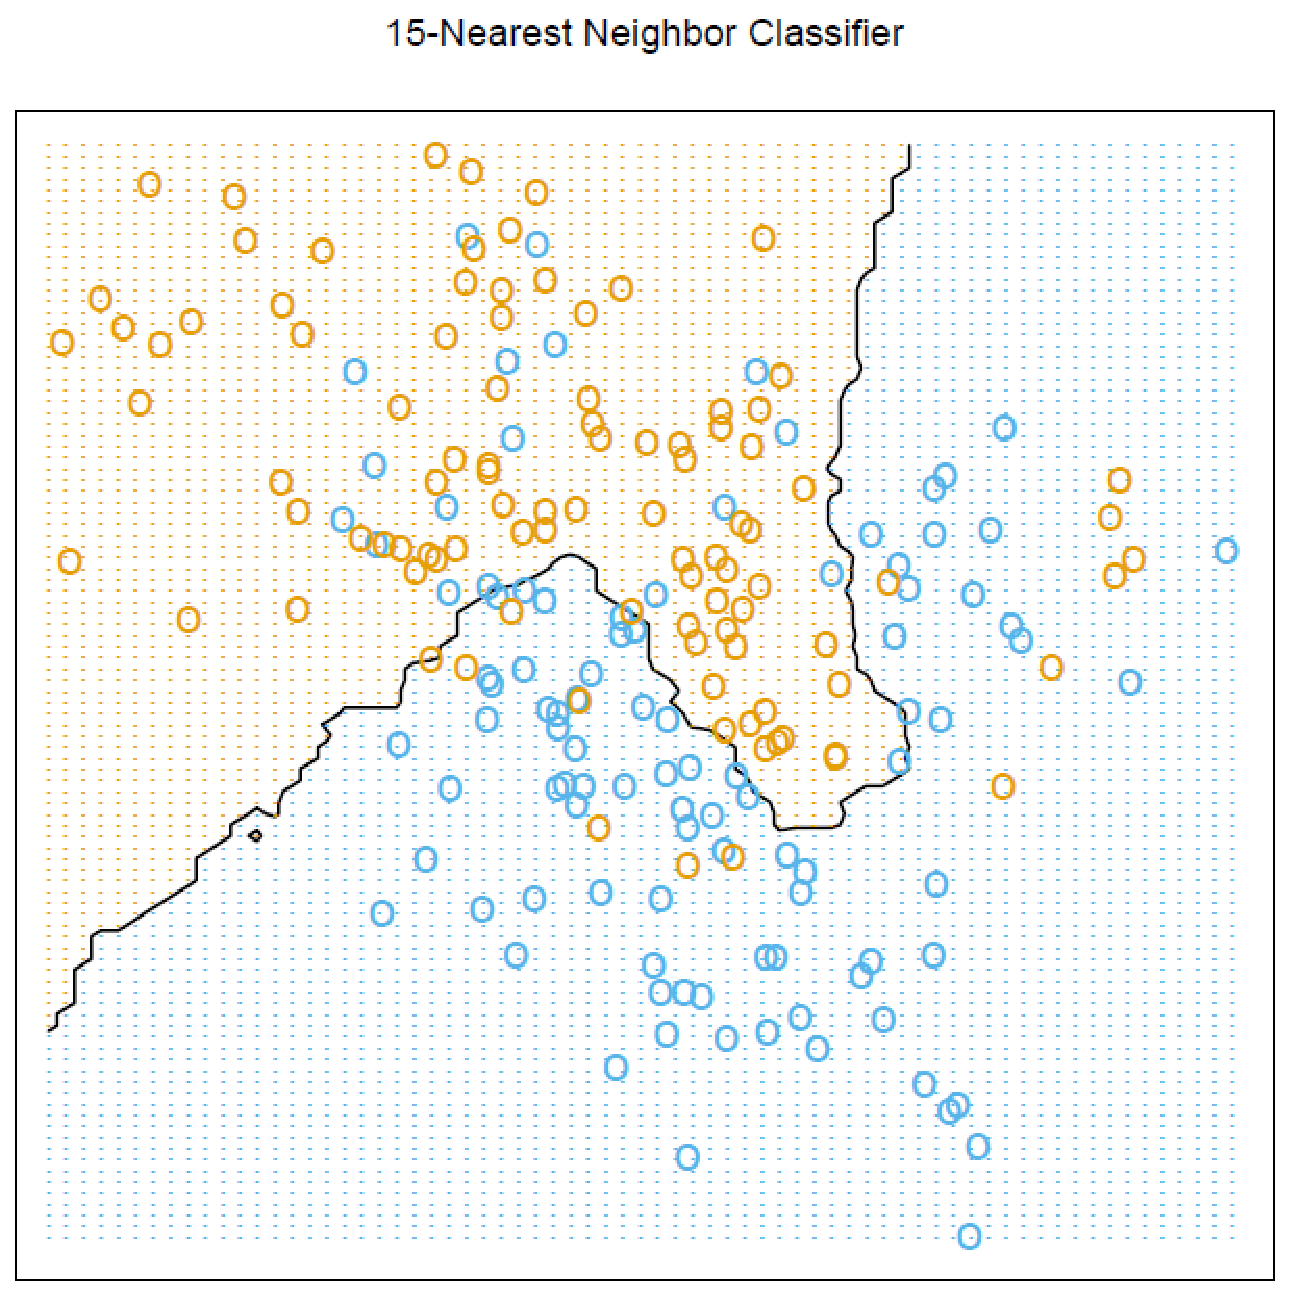
\includegraphics[width=0.8\linewidth]{bound.pdf}
\caption{\label{fig:bound}分界线}
\end{figure}

具体的特征向量系数$\theta$通过最小化成本函数$cost(\theta) = y log(h(\theta x)) + (1-y) log(1-h(\theta x))$
便可获得,这样就得到了逻辑回归分类器。

\subsection{逻辑回归结果}
这里以German Credit的数据为例,表\ref{tab:logit}显示了逻辑回归特征变量系数及其显著性。

\begin{table}[htbp]
  \centering
    \caption{\label{tab:logit}逻辑回归结果}
    \begin{tabular}{lllll}
    \toprule
          & Estimate & Std. Error & z value & $Pr(\ge\|z\|)$ \\
    \midrule
    (Intercept) & -5.48743 & 1.387014 & -3.95629 & 7.61E-05 ***\\
    checking & 0.484832 & 0.089609 & 5.41055 & 6.28E-08 ***\\
    duration & -0.01426 & 0.01144 & -1.24679 & 0.212473 \\
    history & 0.469549 & 0.114837 & 4.088823 & 4.34E-05 ***\\
    purpose & 0.068907 & 0.042475 & 1.622316 & 0.104736 \\
    amount & -0.00015 & 5.07E-05 & -2.99869 & 0.002711 ***\\
    savings & 0.25071 & 0.076253 & 3.287871 & 0.001009 ***\\
    employed & 0.109647 & 0.095728 & 1.145409 & 0.25204 \\
    installp & -0.33189 & 0.106943 & -3.10348 & 0.001913 ***\\
    marital & 0.48904 & 0.155785 & 3.139197 & 0.001694 ***\\
    coapp & 0.100784 & 0.225263 & 0.447406 & 0.654582 \\
    resident & -0.10415 & 0.101927 & -1.02184 & 0.306856 \\
    property & -0.14986 & 0.12051 & -1.24353 & 0.213674 \\
    age   & 0.019083 & 0.011009 & 1.73332 & 0.083039 *\\
    other & 0.325128 & 0.140454 & 2.314837 & 0.020622 **\\
    housing & 0.274481 & 0.216319 & 1.268869 & 0.204488 \\
    existcr & -0.39916 & 0.203087 & -1.96544 & 0.049364 **\\
    job   & 0.34085 & 0.179191 & 1.902159 & 0.057150 *\\
    depends & -0.24825 & 0.290759 & -0.8538 & 0.393214 \\
    telephon & 0.021655 & 0.244287 & 0.088645 & 0.929364 \\
    foreign & 1.699978 & 0.891746 & 1.906348 & 0.056605 *\\
    \bottomrule
    \end{tabular}%
  \label{tab:logit}%
\end{table}%

除此之外,对于拒绝给予贷款的申请人我们给出了三项最有可能导致被拒的原因,见图\ref{fig:topk}

\begin{figure}
\centering
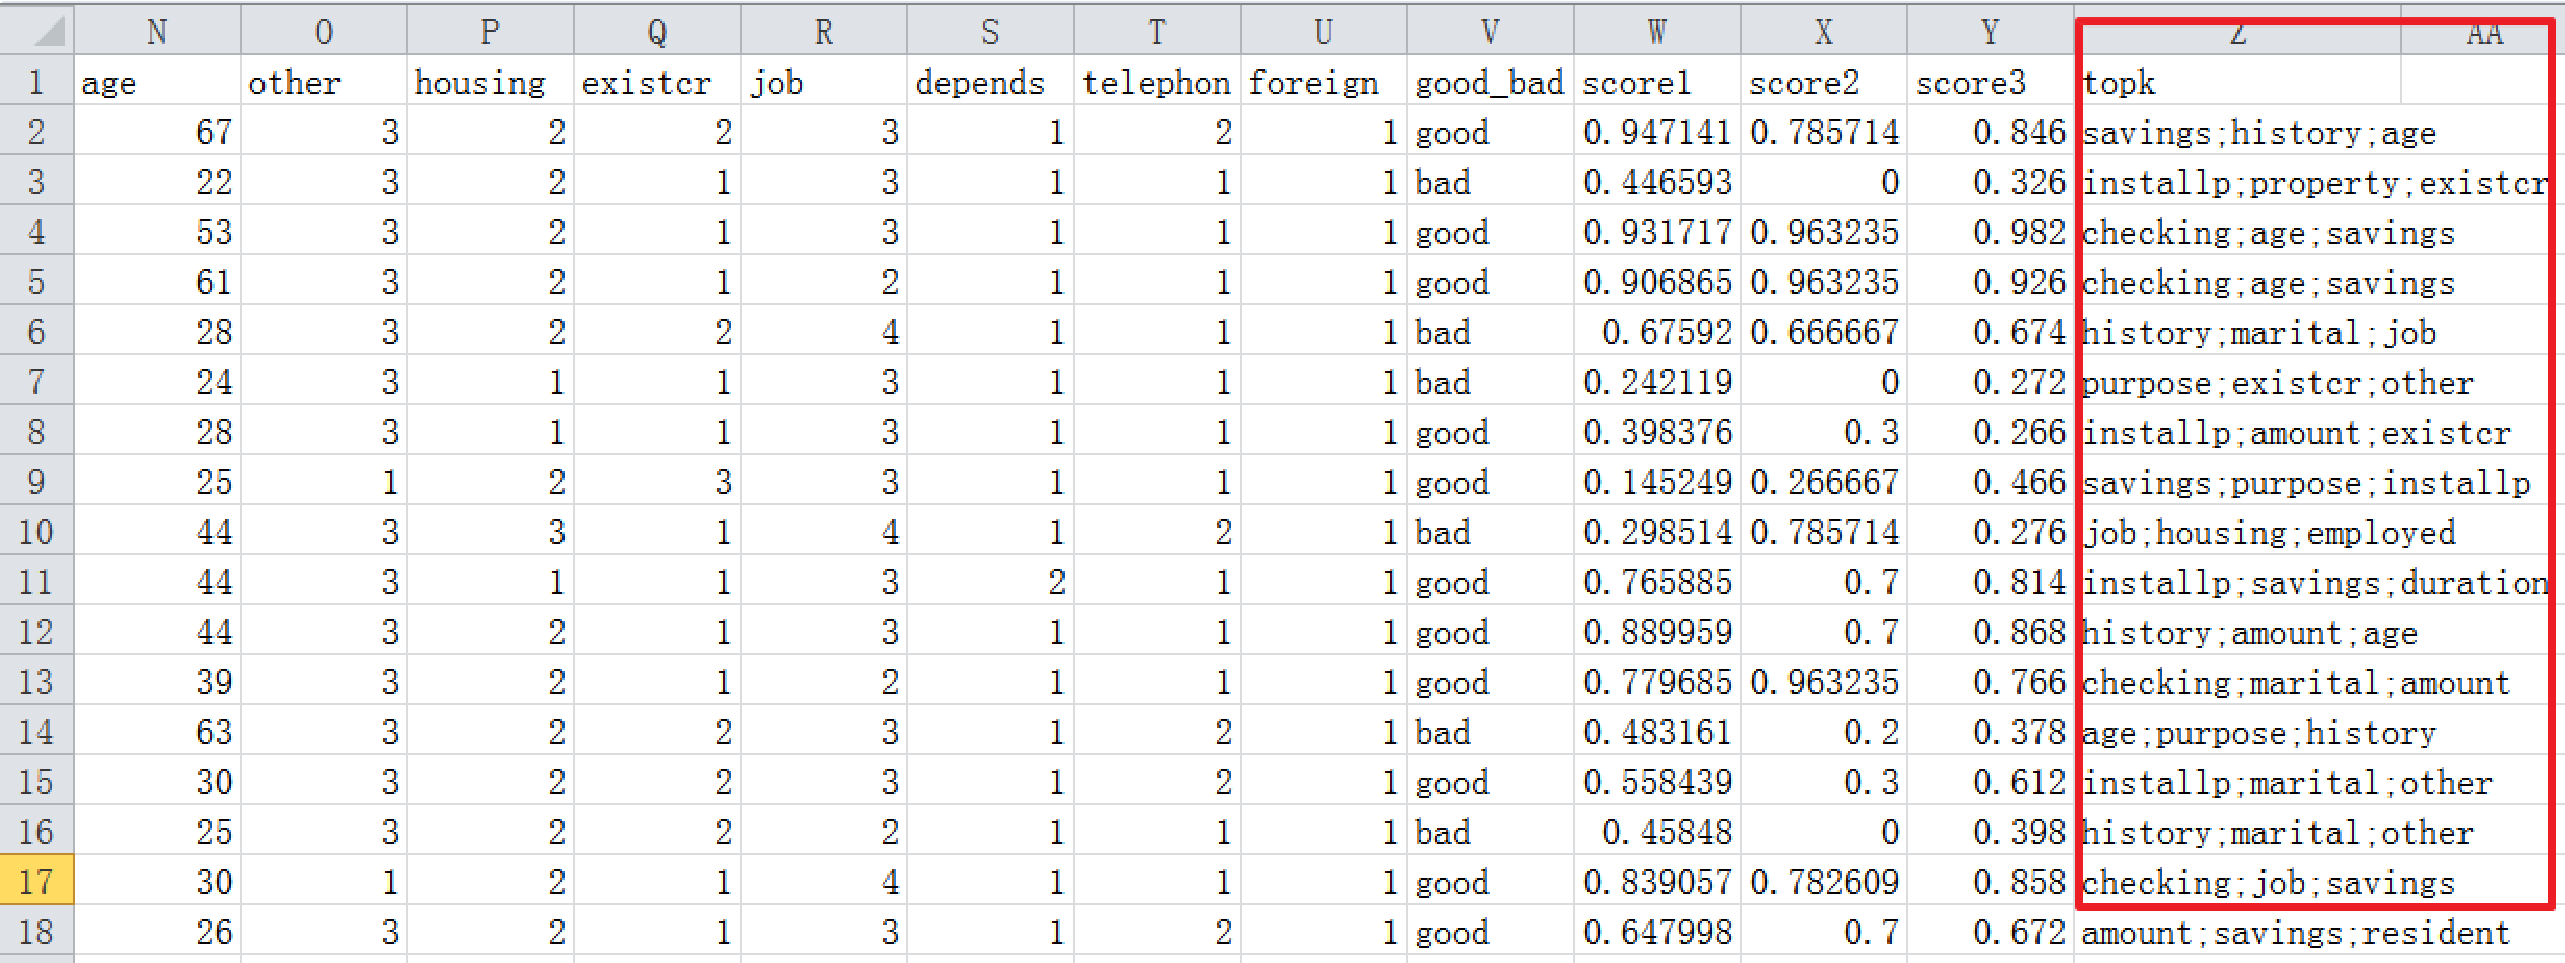
\includegraphics[width=0.8\textwidth]{topk.pdf}
\caption{\label{fig:topk}导致贷款被拒最有可能的三项原因}
\end{figure}

\section{分类树}
\subsection{分类树简介}
分类树通过对数据集按照不同的标准进行分枝,直至无法再分为止。其叶结点表示最终分类结果,其余节点表示各个
分类逻辑表达式。分类树建立的难点在于如何选取分类标准以及相应阈值。传统的ID3是使用信息熵来刻画数据集
的纯度,并选择使得信息增益最大的分类标准作为非叶结点的分裂标准。

\subsection{分类树算法}
数据集$S$的纯度可以用其信息熵来刻画:$H(S) = - \sum _{i} p(i) log(p(i))$,其中$p(i)$表示种类$i$出现的
频率,可见若数据集$S$中的数据只有一类的话,信息熵达到最小值0。其次,非叶节点的分裂标准通过选择使得信息
增益$IG(Y) = H(S) - \sum_{i \in T} p(i) log(p(i))$最大的分类标准(式中子数据集$T$表示按此分类标准
得到的子数据集)。

\subsection{分类树结果}
分类树的结果如图\ref{fig:classification},因为图像显示问题,这里的根节点应为$checking \le 2.5$。
\begin{figure}
\centering
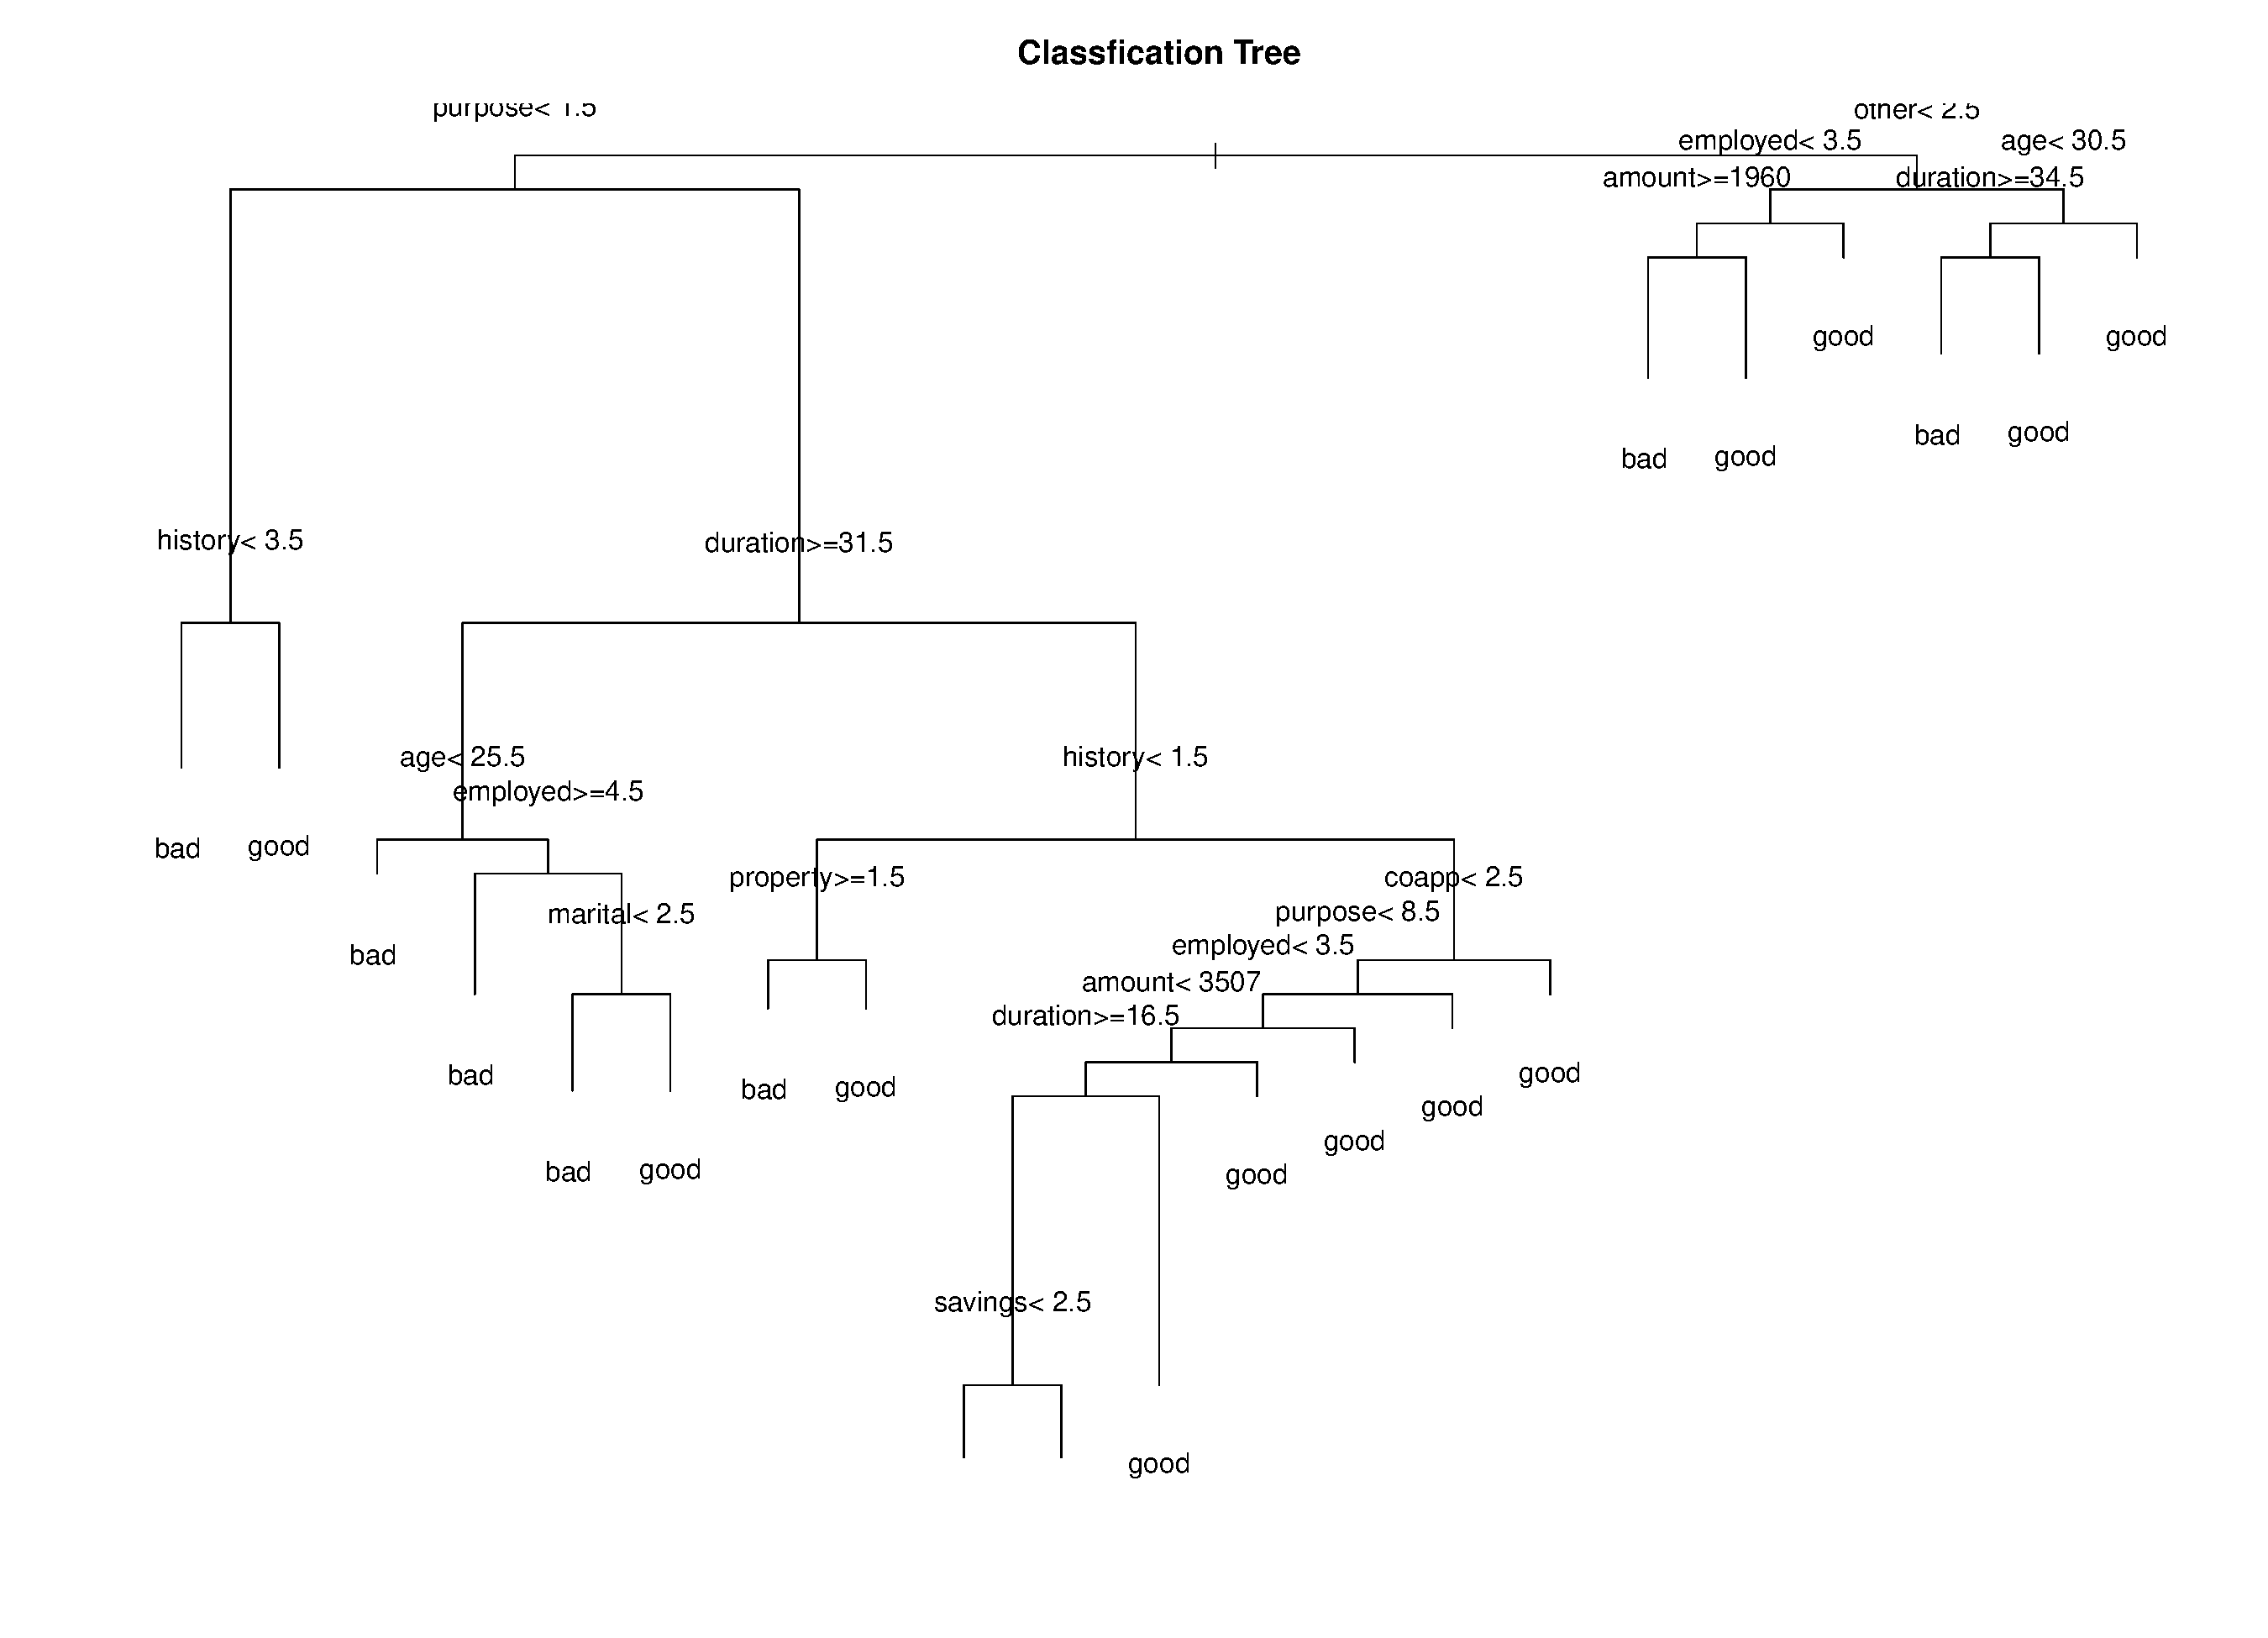
\includegraphics[width=0.8\textwidth]{classificationtree.pdf}
\caption{\label{fig:classification}分类树结果}
\end{figure}

\section{随机森林}

\subsection{随机森林简介}
随机森林是一种集成式学习方法,包含了多个分类树分类器,最终的分类结果由众多分类器投票得出。随机森林因为其
计算效率高、适用于并行处理、可以处理大量数据、评估变量重要性,在最近几年机器学习领域比较流行。微软的体感
游戏设备Kinect也利用了随机森林来识别玩家的动作。

\subsection{随机森林算法}
随机森林是以分类树为基础的集成式学习方法,与其相比,主要有两大区别:
\begin{itemize}
	\item 每棵分类树所使用的数据集是通过自助法对原始数据集进行有放回重取样得到的。
	\item 每棵分类树训练所用的特征变量是随机给定的。
\end{itemize}
最终的分类结果由各棵分类树投票得出。

\subsection{随机森林结果}
随机森林得到的特征变量重要性如图\ref{fig:varimp}
\begin{figure}
\centering
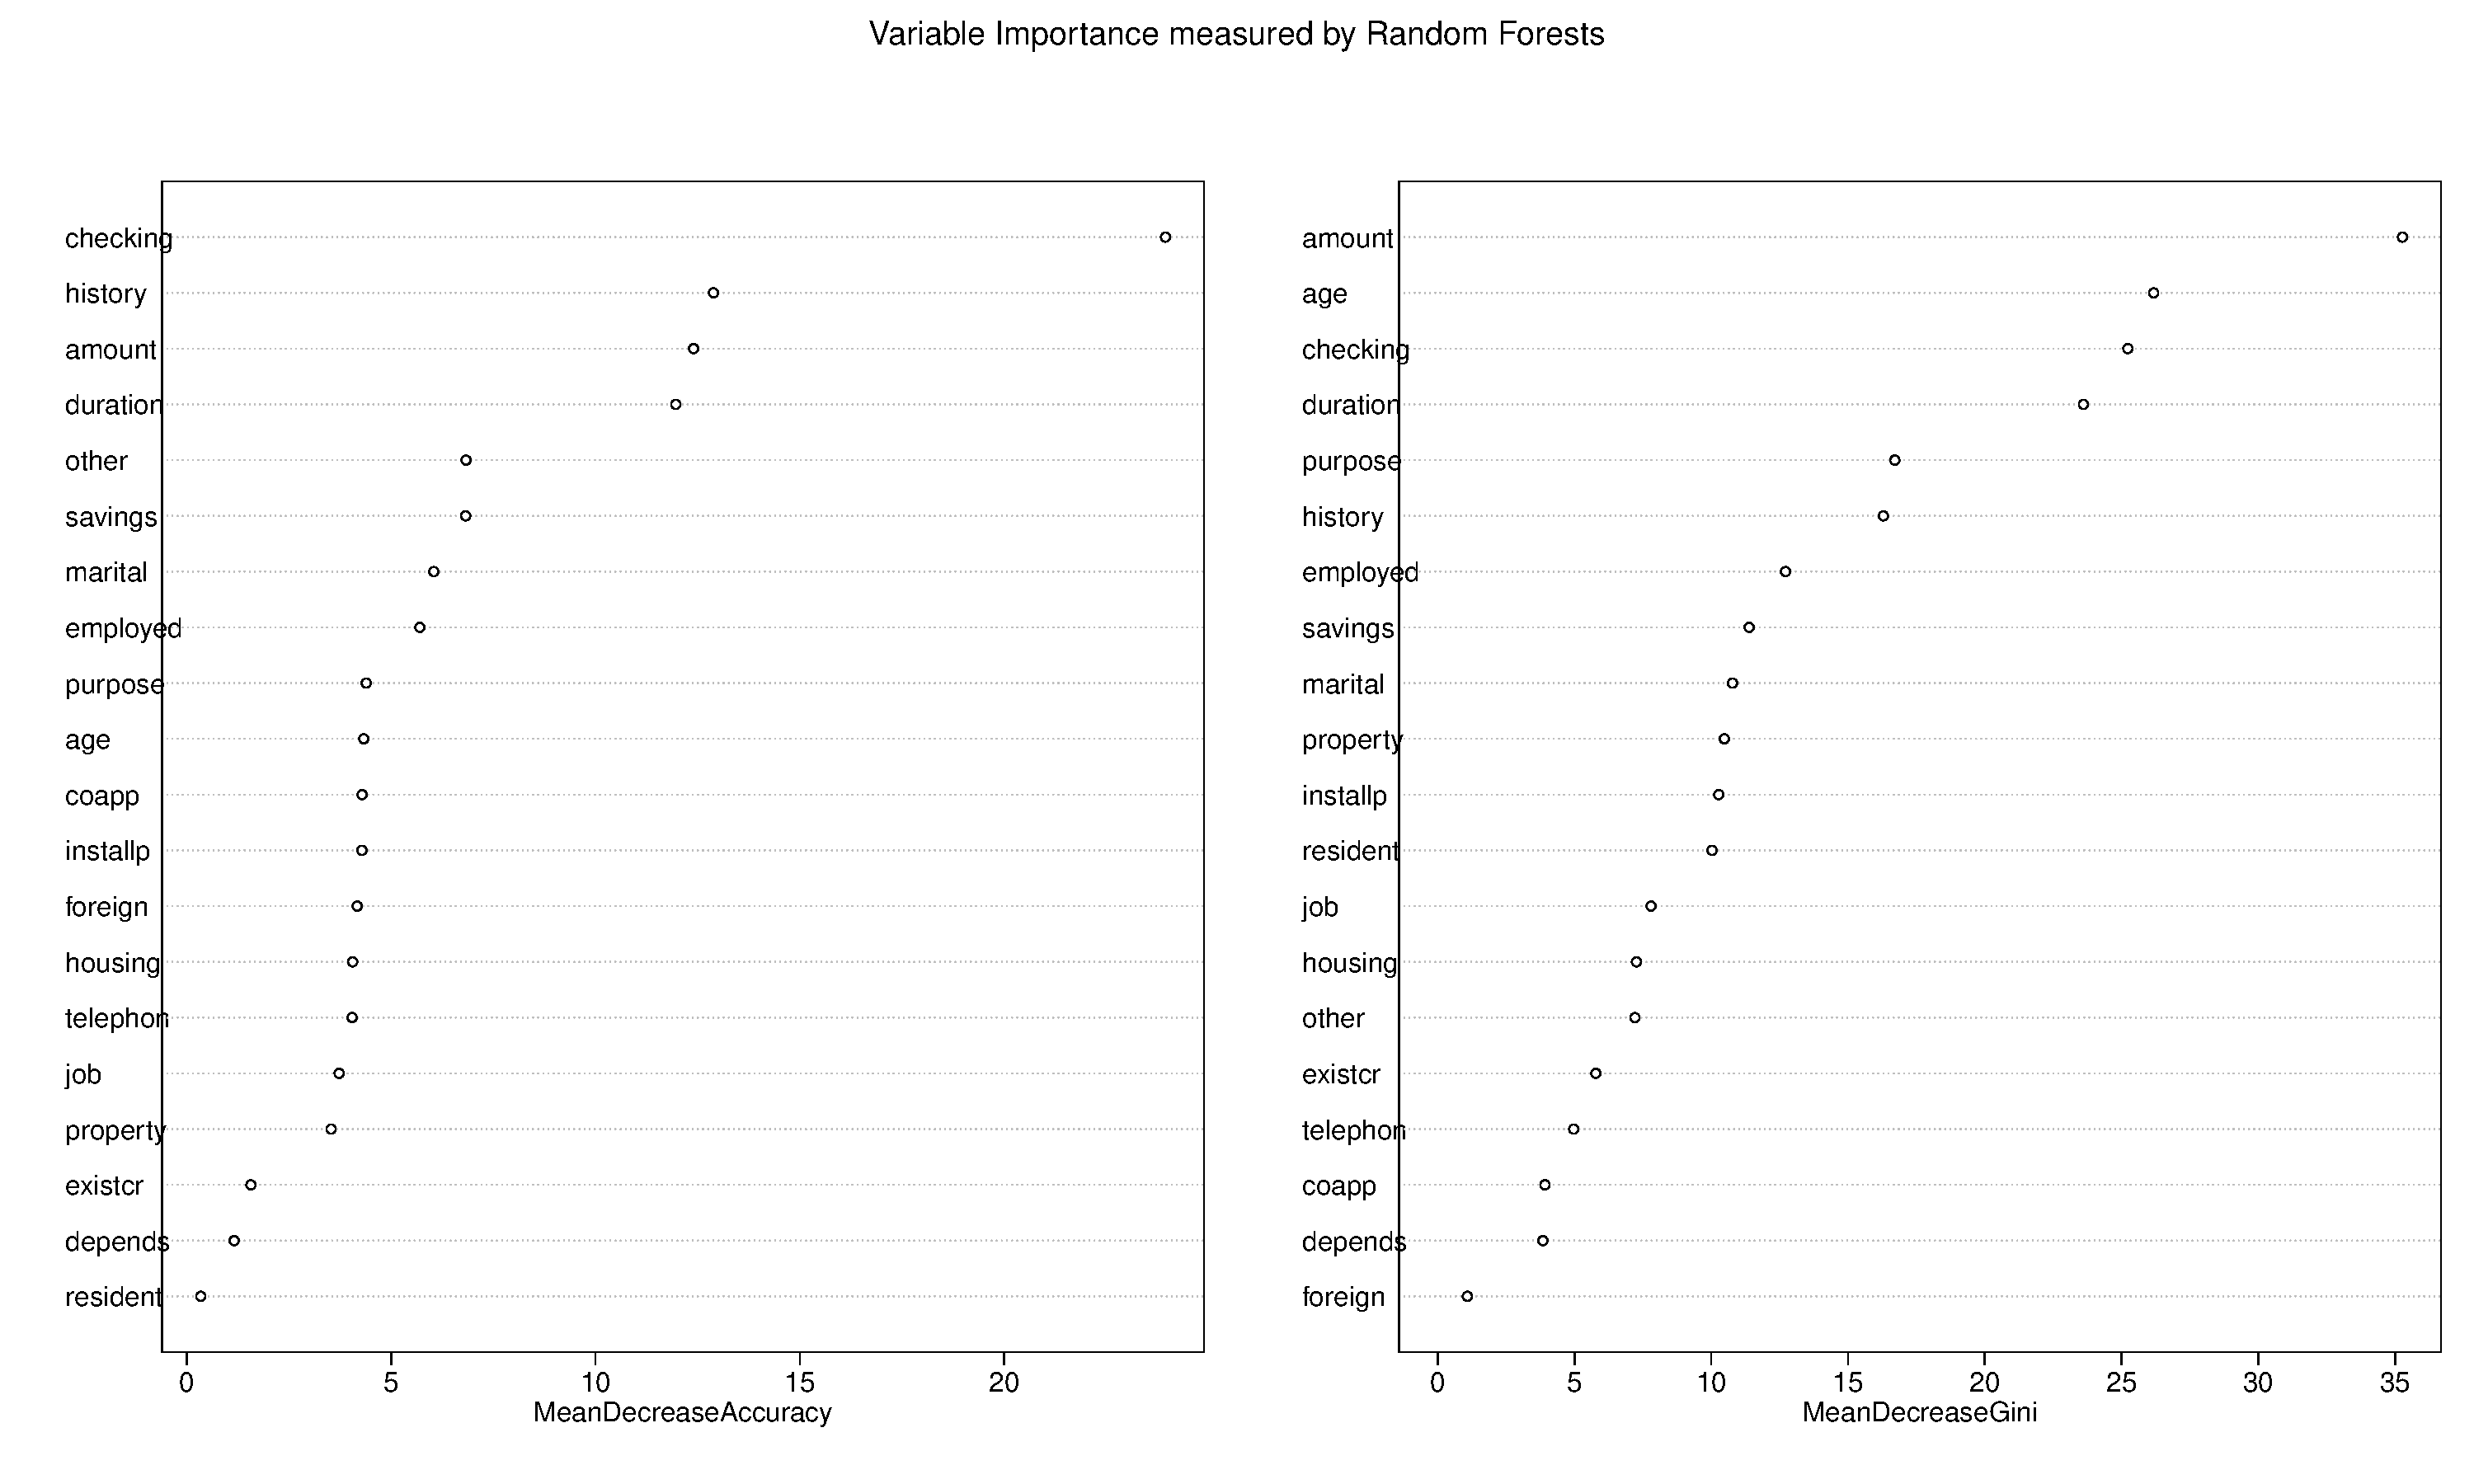
\includegraphics[width=0.8\linewidth]{varimp.pdf}
\caption{\label{fig:varimp}特征变量重要性}
\end{figure}






